% answers.tex —— 2007 年·春季上海卷 · 参考答案与详细解析片段
% 由 tools/generate_projects.py 依来源总账自 2007/2007_数学真题_春季上海_试题.md + 2007/2007_数学真题_春季上海_解析正文.md + 2007/2007_数学真题_春季上海_答案要点.md 生成，勿手改（改源 MD 后重跑）


\begin{gktip}
\textbf{答案说明}：以下为本库依据固定题面独立盲解并经主会话对读整理的非官方推导。源PDF第4–6页印载参考答案仅用于比对，不认证出版者、版次、来源链或官方身份；原文另存归档。Q17为开放题，示例不要求与参考页相同；Q21(3)只选择①。Q20(3)参考页小写角式笔误保留在原文归档，本稿使用独立推导。
\end{gktip}

\begin{answer}
\gksolhead{1}{}

\textbf{题目}（本题满分 $4$ 分）：

计算 $\displaystyle\lim_{n\to\infty}\frac{2n^2+1}{3n(n+1)}=$ $\underline{\qquad\qquad}$。

\Needspace{4\baselineskip}
\textbf{解析}

\Needspace{5\baselineskip}
分子、分母同除以 $n^2$，得

\nopagebreak[4]
\[
\lim_{n\to\infty}\frac{2n^2+1}{3n(n+1)}
=\lim_{n\to\infty}\frac{2+n^{-2}}{3(1+n^{-1})}=\frac23.
\]

\gkanswer{答案：$\dfrac23$。}

\end{answer}
\begin{answer}
\gksolhead{2}{}

\textbf{题目}（本题满分 $4$ 分）：

若关于 $x$ 的一元二次实系数方程 $x^2+px+q=0$ 有一个根为 $1+\mathrm{i}$（$\mathrm{i}$ 是虚数单位），则 $q=$ $\underline{\qquad\qquad}$。

\Needspace{4\baselineskip}
\textbf{解析}

\Needspace{5\baselineskip}
方程的系数为实数，故另一个根为 $1-i$。由韦达定理，

\nopagebreak[4]
\[
q=(1+i)(1-i)=2.
\]

\gkanswer{答案：$q=2$。}

\end{answer}
\begin{answer}
\gksolhead{3}{}

\textbf{题目}（本题满分 $4$ 分）：

若关于 $x$ 的不等式 $\dfrac{x-a}{x+1}>0$ 的解集为 $(-\infty,-1)\cup(4,+\infty)$，则实数 $a=$ $\underline{\qquad\qquad}$。

\Needspace{4\baselineskip}
\textbf{解析}

分母的零点为 $x=-1$，分子的零点为 $x=a$。给定解集的另一有限端点为 $4$，故 $a=4$。

\gkanswer{答案：$a=4$。}

\end{answer}
\begin{answer}
\gksolhead{4}{}

\textbf{题目}（本题满分 $4$ 分）：

函数 $y=(\sin x+\cos x)^2$ 的最小正周期为 $\underline{\qquad\qquad}$。

\Needspace{4\baselineskip}
\textbf{解析}

\Needspace{5\baselineskip}
由恒等式

\nopagebreak[4]
\[
(\sin x+\cos x)^2=1+\sin2x,
\]

可知最小正周期为 $\pi$。

\gkanswer{答案：$\pi$。}

\end{answer}
\begin{answer}
\gksolhead{5}{}

\textbf{题目}（本题满分 $4$ 分）：

设函数 $y=f(x)$ 是奇函数。若 $f(-2)+f(-1)-3=f(1)+f(2)+3$，则 $f(1)+f(2)=$ $\underline{\qquad\qquad}$。

\Needspace{4\baselineskip}
\textbf{解析}

\Needspace{5\baselineskip}
设 $S=f(1)+f(2)$。由奇函数性质，原等式化为

\nopagebreak[4]
\[
-S-3=S+3,
\]

解得 $S=-3$。

\gkanswer{答案：$-3$。}

\end{answer}
\begin{answer}
\gksolhead{6}{}

\textbf{题目}（本题满分 $4$ 分）：

在平面直角坐标系 $xOy$ 中，若抛物线 $y^2=4x$ 上的点 $P$ 到该抛物线的焦点的距离为6，则点 $P$ 的横坐标 $x=$ $\underline{\qquad\qquad}$。

\Needspace{4\baselineskip}
\textbf{解析}

\Needspace{5\baselineskip}
抛物线 $y^2=4x$ 的焦点为 $(1,0)$，准线为 $x=-1$。由抛物线定义，点 $P$ 到焦点的距离等于其到准线的距离，所以

\nopagebreak[4]
\[
x+1=6,
\]

得到横坐标 $x=5$。

\gkanswer{答案：$5$。}

\end{answer}
\begin{answer}
\gksolhead{7}{}

\textbf{题目}（本题满分 $4$ 分）：

在平面直角坐标系 $xOy$ 中，若曲线 $x=\sqrt{4-y^2}$ 与直线 $x=m$ 有且只有一个公共点，则实数 $m=$ $\underline{\qquad\qquad}$。

\Needspace{4\baselineskip}
\textbf{解析}

曲线 $x=\sqrt{4-y^2}$ 是圆 $x^2+y^2=4$ 的右半圆。当 $0\le m<2$ 时，直线 $x=m$ 与曲线有两个交点；当 $m=2$ 时恰有一个交点；其他情形没有交点。因此 $m=2$。

\gkanswer{答案：$2$。}

\end{answer}
\begin{answer}
\gksolhead{8}{}

\textbf{题目}（本题满分 $4$ 分）：

若向量 $\vec a$、$\vec b$ 满足 $|\vec a|=\sqrt2$，$|\vec b|=1$，$\vec a\cdot(\vec a+\vec b)=1$，则向量 $\vec a$、$\vec b$ 的夹角的大小为 $\underline{\qquad\qquad}$。

\Needspace{4\baselineskip}
\textbf{解析}

\Needspace{5\baselineskip}
由已知条件，

\nopagebreak[4]
\[
\vec a\cdot\vec b
=\vec a\cdot(\vec a+\vec b)-|\vec a|^2
=1-2=-1.
\]

\Needspace{5\baselineskip}
设夹角为 $\theta$，则

\nopagebreak[4]
\[
\cos\theta=\frac{\vec a\cdot\vec b}{|\vec a|\,|\vec b|}
=-\frac1{\sqrt2},
\]

所以 $\theta=\dfrac{3\pi}{4}$。

\gkanswer{答案：$\dfrac{3\pi}{4}$，即 $135^\circ$。}

\end{answer}
\begin{answer}
\gksolhead{9}{}

\textbf{题目}（本题满分 $4$ 分）：

若 $x_1$、$x_2$ 为方程 $2^x=\left(\dfrac12\right)^{-\frac1x+1}$ 的两个实数解，则 $x_1+x_2=$ $\underline{\qquad\qquad}$。

\Needspace{4\baselineskip}
\textbf{解析}

\Needspace{5\baselineskip}
原方程要求 $x\ne0$。将右侧化为以 $2$ 为底的幂，比较指数得到

\nopagebreak[4]
\[
x=\frac1x-1,
\qquad x^2+x-1=0.
\]

所得两个实根均非零，由韦达定理，其和为 $-1$。

\gkanswer{答案：$-1$。}

\end{answer}
\begin{answer}
\gksolhead{10}{}

\textbf{题目}（本题满分 $4$ 分）：

在一次教师联欢会上，到会的女教师比男教师多12人，从这些教师中随机挑选一人表演节目。若选到男教师的概率为 $\dfrac9{20}$，则参加联欢会的教师共有 $\underline{\qquad\qquad}$ 人。

\Needspace{4\baselineskip}
\textbf{解析}

\Needspace{5\baselineskip}
设男教师有 $M$ 人，则女教师有 $M+12$ 人，总人数为 $2M+12$。由随机挑选一名教师时选中男教师的概率，

\nopagebreak[4]
\[
\frac{M}{2M+12}=\frac9{20}.
\]

解得 $M=54$，故总人数为 $120$。

\gkanswer{答案：$120$ 人。}

\end{answer}
\begin{answer}
\gksolhead{11}{}

\textbf{题目}（本题满分 $4$ 分）：

函数 $y=\begin{cases}x^2+1,&x\geq0,\\ \dfrac2x,&x<0\end{cases}$ 的反函数是 $\underline{\qquad\qquad}$。

\Needspace{4\baselineskip}
\textbf{解析}

\Needspace{5\baselineskip}
在原函数的非负自变量分支，$y=x^2+1$ 的值域为 $[1,+\infty)$，解得 $x=\sqrt{y-1}$。在负自变量分支，$y=\dfrac2x$ 的值域为 $(-\infty,0)$，解得 $x=\dfrac2y$。交换自变量、因变量，得到

\nopagebreak[4]
\[
f^{-1}(x)=
\begin{cases}
\sqrt{x-1},&x\ge1,\\
\dfrac2x,&x<0.
\end{cases}
\]

反函数的定义域为 $(-\infty,0)\cup[1,+\infty)$。

\gkanswer{答案：反函数为 $f^{-1}(x)=\begin{cases}\sqrt{x-1},&x\ge1,\\ \dfrac2x,&x<0.\end{cases}$，定义域为 $(-\infty,0)\cup[1,+\infty)$。}

\end{answer}
\begin{answer}
\gksolhead{12}{}

\textbf{题目}（本题满分 $4$ 分）：

若集合 $A=\{1,m^2\}$，$B=\{2,4\}$，则“$m=2$”是“$A\cap B=\{4\}$”的

（A） 充分不必要条件。

（B） 必要不充分条件。

（C） 充要条件。

（D） 既不充分也不必要条件。

[答]（　）

\Needspace{4\baselineskip}
\textbf{解析}

当 $m=2$ 时，$A=\{1,4\}$，从而 $A\cap B=\{4\}$，故条件充分。但 $m=-2$ 时结论也成立，所以条件不必要，选择 A。

\gkanswer{答案：A，充分不必要条件。}

\end{answer}
\begin{answer}
\gksolhead{13}{}

\textbf{题目}（本题满分 $4$ 分）：

如图，平面内的两条相交直线 $OP_1$ 和 $OP_2$ 将该平面分割成四个部分 I、II、III、IV（不包括边界）。若 $\overrightarrow{OP}=a\overrightarrow{OP_1}+b\overrightarrow{OP_2}$，且点 $P$ 落在第III部分，则实数 $a$、$b$ 满足
\nopagebreak[4]
\begin{center}% Q13: source PDF p2; intersecting lines have no arrows.
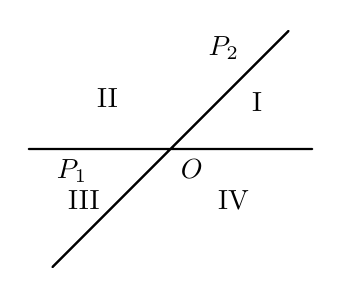
\begin{tikzpicture}[line cap=round,line join=round,thick]
\draw (-1.8,0)--(1.8,0) (-1.5,-1.5)--(1.5,1.5);
\node[below right] at (0,0) {$O$};
\node[below] at (-1.25,0) {$P_1$};
\node[above left] at (1,1) {$P_2$};
\node at (1.1,.6) {I}; \node at (-.8,.65) {II};
\node at (-1.1,-.65) {III}; \node at (.8,-.65) {IV};
\end{tikzpicture}
\end{center}
\nopagebreak[4]
（A） $a>0,b>0$。

（B） $a>0,b<0$。

（C） $a<0,b>0$。

（D） $a<0,b<0$。

[答]（　）

\Needspace{4\baselineskip}
\textbf{解析}

\Needspace{5\baselineskip}
图中第三部分位于 $\overrightarrow{OP_1}$ 的正向与 $\overrightarrow{OP_2}$ 的反向所围成的区域。因此，在

\nopagebreak[4]
\[
\overrightarrow{OP}=a\overrightarrow{OP_1}+b\overrightarrow{OP_2}
\]

中，须有 $a>0$、$b<0$，选择 B。

\gkanswer{答案：B，$a>0$，$b<0$。}

\end{answer}
\begin{answer}
\gksolhead{14}{}

\textbf{题目}（本题满分 $4$ 分）：

下列四个函数中，图象如图所示的只能是

（A） $y=x+\lg x$。

（B） $y=x-\lg x$。

（C） $y=-x+\lg x$。

（D） $y=-x-\lg x$。
\nopagebreak[4]
\begin{center}% Q14: source PDF p2; unticked qualitative curve, no equation label.
\begin{tikzpicture}[line cap=round,line join=round,thick]
\draw[->] (-.45,0)--(3.15,0) node[right] {$x$};
\draw[->] (0,-.45)--(0,2.65) node[above] {$y$};
\draw[domain=-3:.45,samples=150,smooth] plot ({10^(\x)},{.65*(10^(\x)-\x)});
\node[below left] at (0,0) {$O$};
\end{tikzpicture}
\end{center}
\nopagebreak[4]
[答]（　）

\Needspace{4\baselineskip}
\textbf{解析}

图像在 $x\to0^+$ 时趋于 $+\infty$，先减后增，且在 $x\to+\infty$ 时趋于 $+\infty$。四个选项中，$y=x-\lg x$ 具有这些特征，选择 B。

\gkanswer{答案：B，$y=x-\lg x$。}

\end{answer}
\begin{answer}
\gksolhead{15}{}

\textbf{题目}（本题满分 $4$ 分）：

设 $a$、$b$ 是正实数，以下不等式

① $\sqrt{ab}>\dfrac{2ab}{a+b}$，② $a>|a-b|-b$，③ $a^2+b^2>4ab-3b^2$，④ $ab+\dfrac2{ab}>2$ 恒成立的序号为

（A） ①、③。

（B） ①、④。

（C） ②、③。

（D） ②、④。

[答]（　）

\Needspace{4\baselineskip}
\textbf{解析}

\Needspace{5\baselineskip}
对于正数 $a,b$，②等价于 $a+b>|a-b|$，恒成立。④由基本不等式，

\nopagebreak[4]
\[
ab+\frac2{ab}\ge2\sqrt2>2,
\]

也恒成立。①在 $a=b$ 时取等号，不满足严格不等式；③等价于 $(a-2b)^2>0$，在 $a=2b$ 时不成立。因此选择 D。

\gkanswer{答案：D，②、④。}

\end{answer}
\begin{answer}
\gksolhead{16}{}

\textbf{题目}（本题满分 $12$ 分）：

如图，在棱长为2的正方体 $ABCD-A'B'C'D'$ 中，$E$、$F$ 分别是 $A'B'$ 和 $AB$ 的中点，求异面直线 $A'F$ 与 $CE$ 所成角的大小（结果用反三角函数值表示）。
\nopagebreak[4]
\begin{center}% Q16: source PDF p2; hidden AD, DC, DD' and EC dashed.
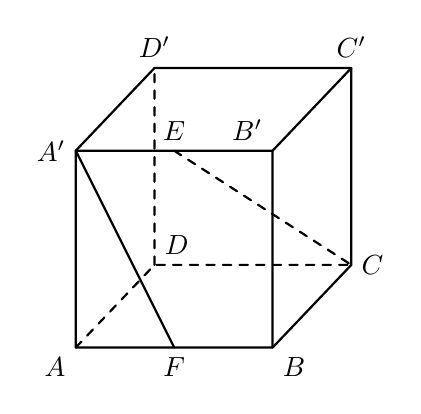
\begin{tikzpicture}[line cap=round,line join=round,thick]
\coordinate (A) at (0,0); \coordinate (B) at (2.5,0);
\coordinate (C) at (3.5,1.05); \coordinate (D) at (1,1.05);
\coordinate (Ap) at (0,2.5); \coordinate (Bp) at (2.5,2.5);
\coordinate (Cp) at (3.5,3.55); \coordinate (Dp) at (1,3.55);
\coordinate (E) at (1.25,2.5); \coordinate (F) at (1.25,0);
\draw[dashed] (A)--(D)--(C) (D)--(Dp) (E)--(C);
\draw (A)--(B)--(C)--(Cp)--(Dp)--(Ap)--cycle;
\draw (Ap)--(Bp)--(Cp) (B)--(Bp) (Ap)--(F);
\node[below left] at (A) {$A$}; \node[below right] at (B) {$B$};
\node[right] at (C) {$C$}; \node[above right] at (D) {$D$};
\node[left] at (Ap) {$A'$}; \node[above left] at (Bp) {$B'$};
\node[above] at (Cp) {$C'$}; \node[above] at (Dp) {$D'$};
\node[above] at (E) {$E$}; \node[below] at (F) {$F$};
\end{tikzpicture}
\end{center}
\nopagebreak[4]
\Needspace{4\baselineskip}
\textbf{解析}

\Needspace{5\baselineskip}
取 $A=(0,0,0)$、$B=(2,0,0)$、$D=(0,2,0)$、$A'=(0,0,2)$，则 $C=(2,2,0)$、$E=(1,0,2)$、$F=(1,0,0)$。两直线的方向向量为
\nopagebreak[4]
\[
\overrightarrow{A'F}=(1,0,-2),\qquad \overrightarrow{CE}=(-1,-2,2).
\]
\Needspace{5\baselineskip}
设异面直线所成角为 $\theta$，按锐角取值，则
\nopagebreak[4]
\[
\cos\theta=\frac{|\overrightarrow{A'F}\cdot\overrightarrow{CE}|}{|\overrightarrow{A'F}|\,|\overrightarrow{CE}|}
=\frac{|-1-4|}{\sqrt5\cdot3}=\frac{\sqrt5}{3}.
\]
所以 $\theta=\arccos\dfrac{\sqrt5}{3}$。

\gkanswer{答案：$\theta=\arccos\dfrac{\sqrt5}{3}$。}

\end{answer}
\begin{answer}
\gksolhead{17}{}

\textbf{题目}（本题满分 $14$ 分）：

求出一个数学问题的正确结论后，将其作为条件之一，提出与原来问题有关的新问题，我们把它称为原来问题的一个“逆向”问题。

例如，原来问题是“若正四棱锥底面边长为4，侧棱长为3，求该正四棱锥的体积”。求出体积 $\dfrac{16}3$ 后，它的一个“逆向”问题可以是“若正四棱锥底面边长为4，体积为 $\dfrac{16}3$，求侧棱长”；也可以是“若正四棱锥的体积为 $\dfrac{16}3$，求所有侧面面积之和的最小值”。

试给出问题“在平面直角坐标系 $xOy$ 中，求点 $P(2,1)$ 到直线 $3x+4y=0$ 的距离”的一个有意义的“逆向”问题，并解答你所给出的“逆向”问题。

\Needspace{4\baselineskip}
\textbf{解析}

\Needspace{5\baselineskip}
原问题中点到直线的距离为

\nopagebreak[4]
\[
\frac{|3\cdot2+4\cdot1|}{\sqrt{3^2+4^2}}=2.
\]

据此构造逆向问题：“点 $P(2,1)$ 到直线 $3x+4y=t$ 的距离为 $2$，求实数 $t$。”

\Needspace{5\baselineskip}
运用点到直线的距离公式，得到

\nopagebreak[4]
\[
\frac{|10-t|}{5}=2.
\]

解得 $t=0$ 或 $t=20$。该问题将原问题得到的距离作为条件，反求直线参数。

\gkanswer{答案：一个有意义的逆向问题是“点 $P(2,1)$ 到直线 $3x+4y=t$ 的距离为 $2$，求实数 $t$”；其解为 $t=0$ 或 $t=20$。}

\end{answer}
\begin{answer}
\gksolhead{18}{}

\textbf{题目}（本题满分 $14$ 分）：

本题共有2个小题，第1小题满分6分，第2小题满分8分。

如图，在直角坐标系 $xOy$ 中，设椭圆 $C:\dfrac{x^2}{a^2}+\dfrac{y^2}{b^2}=1$（$a>b>0$）的左右两个焦点分别为 $F_1$、$F_2$。过右焦点 $F_2$ 且与 $x$ 轴垂直的直线 $l$ 与椭圆 $C$ 相交，其中一个交点为 $M(\sqrt2,1)$。

(1) 求椭圆 $C$ 的方程；

(2) 设椭圆 $C$ 的一个顶点为 $B(0,-b)$，直线 $BF_2$ 交椭圆 $C$ 于另一点 $N$，求 $\triangle F_1BN$ 的面积。
\nopagebreak[4]
\begin{center}% Q18: source PDF p3; only the source's F1,F2,O,M,l labels.
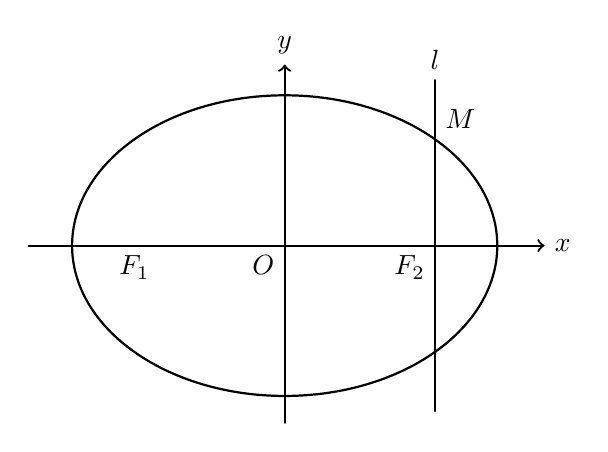
\begin{tikzpicture}[line cap=round,line join=round,thick]
\draw[->] (-3.25,0)--(3.3,0) node[right] {$x$};
\draw[->] (0,-2.25)--(0,2.3) node[above] {$y$};
\draw (0,0) ellipse (2.7 and 1.9092);
\draw (1.9092,-2.1)--(1.9092,2.1) node[above] {$l$};
\node[below left] at (0,0) {$O$};
\node[below] at (-1.9092,0) {$F_1$};
\node[below left] at (1.9092,0) {$F_2$};
\node[above right] at (1.9092,1.35) {$M$};
\end{tikzpicture}
\end{center}
\nopagebreak[4]
\Needspace{4\baselineskip}
\textbf{解析}

\gksubpart{(1) 求椭圆方程}

\Needspace{5\baselineskip}
右焦点的横坐标为 $\sqrt2$，所以 $c^2=2$，即 $a^2-b^2=2$。将点 $M(\sqrt2,1)$ 代入椭圆方程，有

\nopagebreak[4]
\[
\frac2{a^2}+\frac1{b^2}=1.
\]

\Needspace{5\baselineskip}
令 $b^2=t>0$，则

\nopagebreak[4]
\[
\frac2{t+2}+\frac1t=1,
\qquad t^2-t-2=0.
\]

\Needspace{5\baselineskip}
取正根得 $b^2=2$，进而 $a^2=4$，所以椭圆方程为

\nopagebreak[4]
\[
\frac{x^2}{4}+\frac{y^2}{2}=1.
\]

\gksubpart{(2) 求三角形面积}

\Needspace{5\baselineskip}
由第 (1) 问，

\nopagebreak[4]
\[
F_1=(-\sqrt2,0),\quad F_2=(\sqrt2,0),\quad B=(0,-\sqrt2).
\]

\Needspace{5\baselineskip}
直线 $BF_2$ 的方程为 $y=x-\sqrt2$。与椭圆方程联立，化简得

\nopagebreak[4]
\[
x(3x-4\sqrt2)=0.
\]

\Needspace{5\baselineskip}
除点 $B$ 外，另一交点为

\nopagebreak[4]
\[
N=\left(\frac{4\sqrt2}{3},\frac{\sqrt2}{3}\right).
\]

\Needspace{5\baselineskip}
因此

\nopagebreak[4]
\[
\overrightarrow{BF_1}=(-\sqrt2,\sqrt2),\qquad
\overrightarrow{BN}=\left(\frac{4\sqrt2}{3},\frac{4\sqrt2}{3}\right),
\]

\Needspace{5\baselineskip}
面积为

\nopagebreak[4]
\[
S_{\triangle F_1BN}
=\frac12\left|(-\sqrt2)\frac{4\sqrt2}{3}
-\sqrt2\frac{4\sqrt2}{3}\right|
=\frac83.
\]

\gkanswer{答案（1）：$\dfrac{x^2}{4}+\dfrac{y^2}{2}=1$。}

\gkanswer{答案（2）：$S_{\triangle F_1BN}=\dfrac83$。}

\end{answer}
\begin{answer}
\gksolhead{19}{}

\textbf{题目}（本题满分 $14$ 分）：

本题共有2个小题，第1小题满分4分，第2小题满分10分。

某人定制了一批地砖。每块地砖（如图1所示）是边长为0.4米的正方形 $ABCD$，点 $E$、$F$ 分别在边 $BC$ 和 $CD$ 上，$\triangle CFE$、$\triangle ABE$ 和四边形 $AEFD$ 均由单一材料制成，制成 $\triangle CFE$、$\triangle ABE$ 和四边形 $AEFD$ 的三种材料的每平方米价格之比依次为 $3:2:1$。若将此种地砖按图2所示的形式铺设，能使中间的深色阴影部分成四边形 $EFGH$。

(1) 求证：四边形 $EFGH$ 是正方形；

(2) $E$、$F$ 在什么位置时，定制这批地砖所需的材料费用最省？
\nopagebreak[4]
\begin{center}% Q19: source PDF p3; one tile and its four rotated copies.
% Coordinates are schematic and introduce no numerical labels.
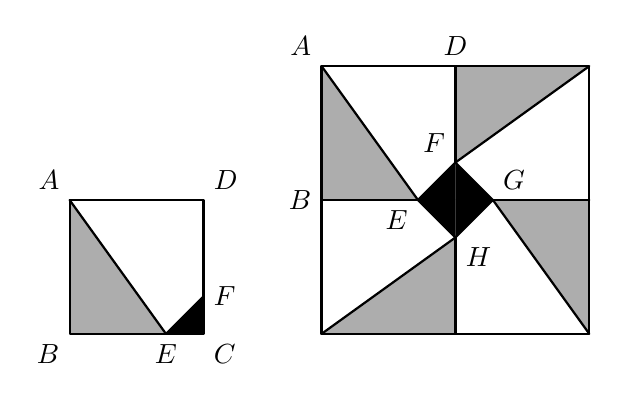
\begin{tikzpicture}[line cap=round,line join=round,thick]
\begin{scope}[scale=1.7]
  \fill[black!32] (0,1)--(0,0)--(.72,0)--cycle;
  \fill[black] (1,0)--(1,.28)--(.72,0)--cycle;
  \draw (0,0) rectangle (1,1); \draw (0,1)--(.72,0)--(1,.28);
  \node[above left] at (0,1) {$A$}; \node[below left] at (0,0) {$B$};
  \node[below right] at (1,0) {$C$}; \node[above right] at (1,1) {$D$};
  \node[below] at (.72,0) {$E$}; \node[right] at (1,.28) {$F$};
\end{scope}
\begin{scope}[xshift=3.2cm,scale=1.7]
  \foreach \angle in {0,90,180,270}{
    \begin{scope}[shift={(1,1)},rotate=\angle,shift={(-1,-1)}]
      \fill[black!32] (0,2)--(0,1)--(.72,1)--cycle;
      \fill[black] (1,1)--(1,1.28)--(.72,1)--cycle;
      \draw (0,2)--(.72,1)--(1,1.28);
    \end{scope}
  }
  \draw (0,0) rectangle (2,2);
  \draw (0,1)--(.72,1) (1.28,1)--(2,1) (1,0)--(1,.72) (1,1.28)--(1,2);
  \node[above left] at (0,2) {$A$}; \node[left] at (0,1) {$B$};
  \node[above] at (1,2) {$D$};
  \node[below left] at (.72,1) {$E$}; \node[above left] at (1,1.28) {$F$};
  \node[above right] at (1.28,1) {$G$}; \node[below right] at (1,.72) {$H$};
\end{scope}
\end{tikzpicture}
\end{center}
\nopagebreak[4]
\Needspace{4\baselineskip}
\textbf{解析}

\gksubpart{(1) 证明中央四边形为正方形}

设砖边长 $s=0.4$ 米，$BE=x$、$CF=y$。四块相同砖按图相邻旋转 $90^\circ$，中央深色阴影恰为四边形，故斜边在各条砖缝处必须接于同一点。

以四砖公共顶点 $O$（左上砖的 $C$）为原点，令 $u=CE=s-x$、$v=CF=y$。左上砖深色三角形的轴端为 $E=(-u,0)$、$F=(0,v)$；相邻砖旋转后的轴端为 $(0,u)$、$(v,0)$。北向顶点 $F$ 是两条斜边的公共端点，因此 $(0,u)=(0,v)$，即 $CE=CF$、$x+y=s$。若两端点不重合，砖缝上多出的边界会使中央阴影成为八边轮廓；等长关系来自拼铺接点与题述四边形约束，不是图片比例或单凭点在边上。

于是 $E=(-y,0)$、$F=(0,y)$、$G=(y,0)$、$H=(0,-y)$，四边等长且邻边垂直，故非退化的 $EFGH$ 是正方形。

\gksubpart{(2) 求材料费用最省时的位置}

\Needspace{5\baselineskip}
设三种材料单价为 $3k,2k,k$（$k>0$）。由 $y=s-x$，两块三角形面积为 $S_{\triangle CFE}=y^2/2$、$S_{\triangle ABE}=sx/2$，所以单砖费用
\nopagebreak[4]
\[
\begin{aligned}
K&=k\left[s^2+2S_{\triangle CFE}+S_{\triangle ABE}\right]
 =k\left[s^2+(s-x)^2+\frac{sx}{2}\right]\\
 &=k\left[\left(x-\frac{3s}{4}\right)^2+\frac{23s^2}{16}\right].
\end{aligned}
\]
当 $BE=x=3s/4=0.3$ 米时费用唯一最小，此时 $CE=CF=s/4=0.1$ 米，$DF=0.3$ 米。

\gkanswer{答案（1）：四边形 $EFGH$ 为正方形。}

\gkanswer{答案（2）：$BE=0.3$ 米、$EC=CF=0.1$ 米、$DF=0.3$ 米时，材料费用最省。}

\end{answer}
\begin{answer}
\gksolhead{20}{}

\textbf{题目}（本题满分 $18$ 分）：

本题共有3个小题，第1小题满分6分，第2小题满分4分，第3小题满分8分。

通常用 $a$、$b$、$c$ 分别表示 $\triangle ABC$ 的三个内角 $A$、$B$、$C$ 所对边的边长，$R$ 表示 $\triangle ABC$ 的外接圆半径。

(1) 如图，在以 $O$ 为圆心、半径为2的 $\odot O$ 中，$BC$ 和 $BA$ 是 $\odot O$ 的弦，其中 $BC=2$，$\angle ABC=45^\circ$，求弦 $AB$ 的长；

(2) 在 $\triangle ABC$ 中，若 $\angle C$ 是钝角，求证：$a^2+b^2<4R^2$；

(3) 给定三个正实数 $a$、$b$、$R$，其中 $b\leq a$。问：$a$、$b$、$R$ 满足怎样的关系时，以 $a$、$b$ 为边长、$R$ 为外接圆半径的 $\triangle ABC$ 不存在、存在一个或存在两个（全等三角形算作同一个）？在 $\triangle ABC$ 存在的情况下，用 $a$、$b$、$R$ 表示 $c$。
\nopagebreak[4]
\begin{center}% Q20: source PDF p3; only BA and BC, AB is not a diameter.
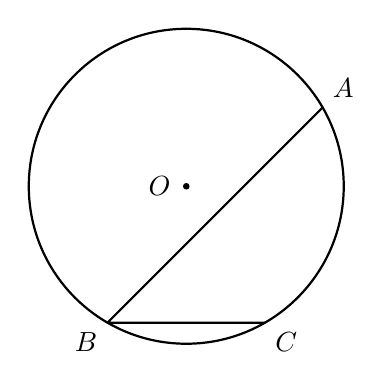
\begin{tikzpicture}[line cap=round,line join=round,thick]
\coordinate (O) at (0,0);
\coordinate (A) at (30:2); \coordinate (B) at (240:2); \coordinate (C) at (300:2);
\draw (O) circle[radius=2]; \draw (A)--(B)--(C);
\fill (O) circle[radius=1.2pt]; \node[left=2pt] at (O) {$O$};
\node[above right] at (A) {$A$}; \node[below left] at (B) {$B$};
\node[below right] at (C) {$C$};
\end{tikzpicture}
\end{center}
\nopagebreak[4]
\Needspace{4\baselineskip}
\textbf{解析}

\gksubpart{(1) 求弦长}

\Needspace{5\baselineskip}
由正弦定理和 $BC=2$、$R=2$，

\nopagebreak[4]
\[
\sin A=\frac{BC}{2R}=\frac12.
\]

\Needspace{5\baselineskip}
因 $B=45^\circ$，不能取 $A=150^\circ$，故 $A=30^\circ$、$C=105^\circ$。再次应用正弦定理，

\nopagebreak[4]
\[
AB=4\sin105^\circ=\sqrt6+\sqrt2.
\]

\gksubpart{(2) 证明不等式}

\Needspace{5\baselineskip}
当 $C$ 为钝角时，$A+B<\dfrac\pi2$，且 $|A-B|<\dfrac\pi2$，所以

\nopagebreak[4]
\[
\sin^2A+\sin^2B
=1-\cos(A+B)\cos(A-B)<1.
\]

\Needspace{5\baselineskip}
由 $a=2R\sin A$、$b=2R\sin B$，得到

\nopagebreak[4]
\[
a^2+b^2=4R^2(\sin^2A+\sin^2B)<4R^2.
\]

\gksubpart{(3) 讨论存在性并表示第三边}

已知 $0<b\le a$、$R>0$。若 $a>2R$，正弦定理将要求 $\sin A>1$，故不存在三角形。

\Needspace{5\baselineskip}
当 $a\le2R$ 时，令

\nopagebreak[4]
\[
\alpha=\arcsin\frac{a}{2R},\qquad
\beta=\arcsin\frac{b}{2R},
\]

有 $0<\beta\le\alpha\le\dfrac\pi2$。角 $A$ 可取 $\alpha$ 或 $\pi-\alpha$，角 $B$ 可取 $\beta$ 或 $\pi-\beta$，同时须满足 $A+B<\pi$。

当 $0<b<a<2R$ 时，合法组合恰为 $(A,B)=(\alpha,\beta)$ 和 $(\pi-\alpha,\beta)$，存在两个三角形。当 $0<b=a<2R$ 时，只能取 $(A,B)=(\alpha,\alpha)$，存在一个三角形。当 $0<b<a=2R$ 时，只能取 $(A,B)=(\dfrac\pi2,\beta)$，也存在一个三角形。当 $a=b=2R$ 时，两个角均为直角，不能构成三角形。

\Needspace{5\baselineskip}
综上，完整分类为

\nopagebreak[4]
\[
\begin{cases}
\text{不存在},&a>2R\text{，或 }a=b=2R,\\
\text{存在一个},&0<b=a<2R\text{，或 }0<b<a=2R,\\
\text{存在两个},&0<b<a<2R.
\end{cases}
\]

\Needspace{5\baselineskip}
对于存在的三角形，由 $C=\pi-A-B$，

\nopagebreak[4]
\[
\begin{aligned}
c&=2R\sin(A+B)\\
 &=a\cos B+b\cos A\\
 &=\frac{a\sqrt{4R^2-b^2}\pm b\sqrt{4R^2-a^2}}{2R}.
\end{aligned}
\]

当 $0<b<a<2R$ 时，两种符号均取：加号对应 $A=\alpha$，减号对应 $A=\pi-\alpha$。当 $0<b=a<2R$ 时只取加号，减号给出退化的 $c=0$。当 $0<b<a=2R$ 时两种表达式重合，均为 $c=\sqrt{4R^2-b^2}$。

固定副本PDF第5页本题参考解中有 $\cos(a+B)$ 的小写字母印载笔误；本解析由正弦定理独立推导第三边，角式使用 $A+B$，不将更正后的式子称为源文逐字转录。

\gkanswer{答案（1）：$AB=\sqrt6+\sqrt2$。}

\gkanswer{答案（2）：$a^2+b^2<4R^2$。}

\gkanswer{答案（3）：在 $0<b\le a$、$R>0$ 下，不存在三角形当且仅当 $a>2R$ 或 $a=b=2R$；存在一个三角形当且仅当 $0<b=a<2R$ 或 $0<b<a=2R$；存在两个三角形当且仅当 $0<b<a<2R$。存在时 $c=\dfrac{a\sqrt{4R^2-b^2}\pm b\sqrt{4R^2-a^2}}{2R}$；$b<a<2R$ 时两种符号均取，$a=b<2R$ 时只取加号，$b<a=2R$ 时两式重合为 $\sqrt{4R^2-b^2}$。}

\end{answer}
\begin{answer}
\gksolhead{21}{}

\textbf{题目}（本题满分 $18$ 分）：

本题共有3个小题，第1小题满分4分，第2小题满分6分，第3小题满分8分。

\Needspace{5\baselineskip}
我们在下面的表格内填写数值：先将第1行的所有空格填上1；再把一个首项为1、公比为 $q$ 的数列 $\{a_n\}$ 依次填入第一列的空格内；然后按照“任意一格的数是它上面一格的数与它左边一格的数之和”的规则填写其它空格。

\nopagebreak[4]
\[
\begin{array}{|c|c|c|c|c|c|}
\hline
 & \text{第1列} & \text{第2列} & \text{第3列} & \cdots & \text{第}n\text{列} \\ \hline
\text{第1行} & 1 & 1 & 1 & \cdots & 1 \\ \hline
\text{第2行} & q & & & & \\ \hline
\text{第3行} & q^2 & & & & \\ \hline
\cdots & \cdots & & & & \\ \hline
\text{第}n\text{行} & q^{n-1} & & & & \\ \hline
\end{array}
\]

(1) 设第2行的数依次为 $B_1,B_2,\cdots,B_n$，试用 $n$、$q$ 表示 $B_1+B_2+\cdots+B_n$ 的值；

(2) 设第3列的数依次为 $c_1,c_2,c_3,\cdots,c_n$，求证：对于任意非零实数 $q$，$c_1+c_3>2c_2$；

(3) 请在以下两个问题中选择一个进行研究（只能选择一个问题，如果都选，被认为选择了第一问）。

① 能否找到 $q$ 的值，使得(2)中的数列 $c_1,c_2,c_3,\cdots,c_n$ 的前 $m$ 项 $c_1,c_2,c_3,\cdots,c_m$（$m\geq3$）成为等比数列？若能找到，$m$ 的值有多少个？若不能找到，说明理由。

② 能否找到 $q$ 的值，使得填完表格后，除第1列外，还有不同的两列数的前三项各自依次成等比数列？并说明理由。

\Needspace{4\baselineskip}
\textbf{解析}

题目使用第3行、第3列，以下在表格包含这些行列的语境下讨论。第1行全为1，首列为 $1,q,q^2,\ldots$，其余按题设“上方与左方之和”递推。

\gksubpart{(1) 求第二行各数之和}

\Needspace{5\baselineskip}
有 $B_1=q$、$B_j=B_{j-1}+1$，故 $B_j=q+j-1$，从而
\nopagebreak[4]
\[
B_1+B_2+\cdots+B_n=nq+\frac{n(n-1)}2.
\]

\gksubpart{(2) 证明第三列前三项满足不等式}

第2行前三项为 $q,q+1,q+2$，第3行第2项为 $q^2+q+1$，所以 $c_1=1$、$c_2=q+2$、$c_3=(q+2)+(q^2+q+1)=q^2+2q+3$。对于任意非零实数 $q$，有 $c_1+c_3-2c_2=q^2>0$，即 $c_1+c_3>2c_2$。

\gksubpart{(3) 仅选择第①问：讨论前若干项成等比数列}

若前 $m$ 项成等比数列且 $m\ge3$，则前三项必须成等比数列。由 $c_1=1$，得 $c_2^2=c_1c_3$，即 $(q+2)^2=q^2+2q+3$，解得 $q=-\dfrac12$。

此时前三项为 $1,\dfrac32,\dfrac94$，确成公比为 $\dfrac32$ 的等比数列。但由递推，第四项 $c_4=q^3+2q^2+3q+4=\dfrac{23}{8}\ne\dfrac{27}{8}=\left(\dfrac32\right)^3$。因此任意 $m\ge4$ 都不可能，满足条件的 $m$ 仅有 $3$ 一个值。

\gkanswer{答案（1）：$B_1+B_2+\cdots+B_n=nq+\dfrac{n(n-1)}2$。}

\gkanswer{答案（2）：$c_1+c_3-2c_2=q^2>0$，所以 $c_1+c_3>2c_2$。}

\gkanswer{答案（3）：仅选择第①问。$q=-\dfrac12$，$m$ 只有一个可能值，即 $m=3$，此时前三项的公比为 $\dfrac32$。}

\end{answer}